
\documentclass[11pt]{article}
\usepackage{standalone}
\usepackage[margin=0.75in, headheight=20pt]{geometry}

\usepackage{amsmath}
\usepackage{amsfonts}
\usepackage{amssymb}
\usepackage{mathtools}

\usepackage{tikz}
\usetikzlibrary{shadings,intersections}

\usepackage{caption,tabularx,booktabs}

\usepackage{rotating}

\usepackage[utf8]{inputenc}
\usepackage[english]{babel}
\setlength{\parindent}{2em}
\setlength{\parskip}{.25em}
\renewcommand{\baselinestretch}{1.0}

\usepackage{fancyhdr}
\pagestyle{fancy}
\rhead{ Clarke | Blostein | Queen's University}
\renewcommand{\headrulewidth}{0.4pt}
\renewcommand{\footrulewidth}{0.4pt}

\usepackage{courier}

\usepackage[]{algorithm2e}
\usepackage{mathrsfs}

\usepackage{etoolbox}
\patchcmd{\thebibliography}{\chapter*}{\section*}{}{}




\title{Performance comparison between unconstrained and SUS-constrained linear MRT beamforming}
\author{J.E. Clarke, Dr. S.D. Blostein | Queen's University}
\date{Fall, 2018}

\begin{document}
	\maketitle
	\newpage
	\section{Introduction and Summary of Results}
	    In this paper results are presented that compare the performance of semi-orthogonal user selection (SUS) scheme assuming MRT beamforming in the MU-MIMO downlink to a brute-force approach to user selection. The brute-force approach represents a computation-intensive exhaustive search for the best performance associated with a group of users chosen from a larger group of candidate users. In this way, the exhaustive search for the best possible performance is a best-case benchmark to compare against the SUS scheme, which reduces the size of the search space, and thus the computational complexity.

The focus of this paper is to compare the performance of the SUS, constrained case, to the exhaustive, unconstrained case; computational complexity will be addressed separately in future work. The performance metric of interest is the sum rate of a group of four users chosen from a larger set of candidate users. The findings presented here suggest that the SUS scheme has a low probability of meeting the exhaustive case. However, as the number of candidate users becomes larger, the SUS constraints do better at filtering the search space. Put differently: as the number of candidate users increases, the probability that the group associated with the best sum rate in the exhaustive search space overlaps with the much smaller SUS-constrained search space. For example, the probability that the SUS search space contains the group with the best sum rate for 30 candidate users is approximately $2\times10^{-4}$. However, as the number of candidate users is increased to 1000, the probability of the such an overlap is increased to 0.13. Thus, as the number of candidate users becomes large, as in the case of a dense wireless deployment, user selection based on channel orthogonality and gain becomes increasingly attractive from a performance point of view. Moreover, the results presented here suggest that lower bound on the expected sum rate approaches the expected maximum sum rate as the number of candidate users becomes large.

The results presented in this paper are conservative. The sum rate results associated with SUS-constrained cases are characterized by lower bounds, while the unconstrained results are not subjected to such lower bounds. 

SUS scheme does not achieve performance as high as the exhaustive search. However, this is neither surprising, nor the argument presented here. The purpose of this effort is to quantify the losses in sum rate performance. Such quantitative analysis is necessary in order to argue a reasonable performance-complexity trade-off.
	\section{Discussion of Results}
	    \subsection{Approach and Interpretation}
Results associated with the SUS-constrained case are shown in Figs. \ref{fig:30_candidate}, \ref{fig:100_candidate}, \ref{fig:1000_candidate}. These plots show lower bound of expected sum rate plotted against the pairwise orthogonality constraint between channels. From these plots it is clear that sum rate as a function of this constraint is a convex function. There is a balance between quantity and quality of users. In the left-hand side of the plots, the requirement is so strict that no users are able to meet it, resulting in low sum rate. In the right-hand side of the plot, users are not sufficiently orthogonal to each other, even though many users and groups of users meet these constraints; again, the result is low sum rate. The maximal sum rate occurs when the orthogonality constraint takes a value between these extremes.

Results associated with the unconstrained, or brute-force case are shown in Figs. \ref{fig:30_candidate_cdf}, \ref{fig:100_candidate_cdf}, \ref{fig:1000_candidate_cdf}. These plots are cumulative probability distributions (CDFs). These CDFs describe the probability of finding a group of a given maximum sum rate by exhaustively searching all combinations of candidate users to form 4-user groups.

A statistical comparison between the constrained and unconstrained spaces is made by taking the maximum constrained sum rate as an argument of the CDF in the unconstrained case. The probability that the exhaustive search achieves a performance greater than the constrained space is equal to 1-$F(C_{SUS})$, where $F(C_{SUS})$ is the CDF probability evaluated at the lower bound on the expected SUS-constrained sum rate. An alternative way of interpreting these results is the probability that the smaller SUS-constrained space contains the group associated with the maximum sum rate.

\subsection{Plots}

Three scenarios were investigated with different number of candidate users: 30, 100, and 1000 candidate users. Each of these cases were investigated with a SNR of 10dB.

The first comparison, for the 30 candidate scenario, is shown in Figs. \ref{fig:30_candidate}, \ref{fig:30_candidate_cdf}. From Fig \ref{fig:30_candidate} we can see that the maximum lower bound on expected sum rate for the SUS-constrained case is 2.3bps/Hz which occurs at an orthogonality constraint of 0.85. From Fig. \ref{fig:30_candidate_cdf}, we can see that the probability of finding a maximum sum rate that exceeds 2.3bps/Hz is nearly 1. We can also see from Fig. \ref{fig:30_candidate_cdf} that we expect to find a maximum sum rate of 5.0bps/Hz in the brute-force search of the unconstrained space. Therefore, on average, there is a factor of 2.2 increase in sum rate performance comparing the lower bound in the constrained case to the unconstrained case.

The second comparison, for the 100 candidate scenario, is shown in Figs. \ref{fig:100_candidate}, \ref{fig:100_candidate_cdf}. From Fig \ref{fig:100_candidate} we can see that the maximum lower bound on expected sum rate for the SUS-constrained case is 4.5bps/Hz which occurs at an orthogonality constraint of 0.82. From Fig. \ref{fig:100_candidate_cdf}, we can see that the probability of finding a maximum sum rate that exceeds 4.5bps/Hz is nearly 1. We can also see from Fig. \ref{fig:100_candidate_cdf} that we expect to find a maximum sum rate of 6.0bps/Hz in the brute-force search of the unconstrained space. Therefore, on average, there is a factor of 1.33 increase in sum rate performance comparing the lower bound in the constrained case to the unconstrained case. This ratio illustrates that the increase in the constrained lower bound has moved further to the right the tail of the unconstrained curve than the mean of this curve has shifted right: the constrained case is catching up to the unconstrained case when the number of candidates was increased.

The second comparison, for the 100 candidate scenario, is shown in Figs. \ref{fig:1000_candidate}, \ref{fig:1000_candidate_cdf}. From Fig \ref{fig:1000_candidate} we can see that the maximum lower bound on expected sum rate for the SUS-constrained case is 7.1bps/Hz which occurs at an orthogonality constraint of 0.61. From Fig. \ref{fig:1000_candidate_cdf}, we can see that the probability of finding a maximum sum rate that exceeds 7.1bps/Hz is no longer nearly 1; instead, there is a probability of 0.87 that the unconstrained approach will result in a higher sum rate than the constrained case. Conversely, there is a probability of 0.13 that the group with the maximum sum rate will overlap the constrained search space. We can also see from Fig. \ref{fig:1000_candidate_cdf} that we expect to find a maximum sum rate of 7.6bps/Hz in the brute-force search of the unconstrained space. Therefore, on average, there is a factor of 1.07 increase in sum rate performance comparing the lower bound in the constrained case to the unconstrained case. The trend previously illustrated continues. Moreover, as the number of candidate users becomes sufficiently large the performance gains associated with the unconstrained case diminish, and the lower bound on the expected sum rate in the constrained case approaches the mean of the unconstrained case.


\begin{figure}
    \centering
    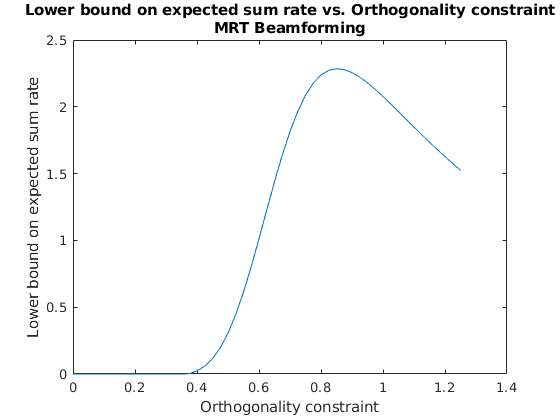
\includegraphics[width=18cm]{figs/30_candidate_rho1_25_mrt.png}\\
    \caption{Sum rate for two-dimensional constellations as a function of pairwise orthogonality requirement between user channels in a given group. Four users per group is assumed, four transmit antennas assumed. Number of candidate STAs for addition to SUS groups is set to 30. SNR 10dB.}
    \label{fig:30_candidate}
\end{figure}

\begin{figure}
    \centering
    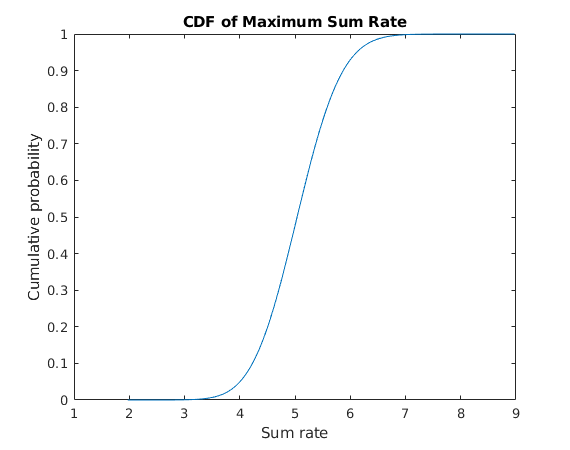
\includegraphics[width=18cm]{figs/cdf_4gs_30cand_1Ptx_0_1Pn.png}\\
    \caption{CDF of maximum sum rate for two-dimensional constellations resulting from exhaustive search of all combinations of user groups chosen from the set of candidate users.  Four users per group is assumed, four transmit antennas assumed. Number of candidate STAs for addition to SUS groups is set to 30. SNR 10dB.}
    \label{fig:30_candidate_cdf}
\end{figure}

\begin{figure}
    \centering
    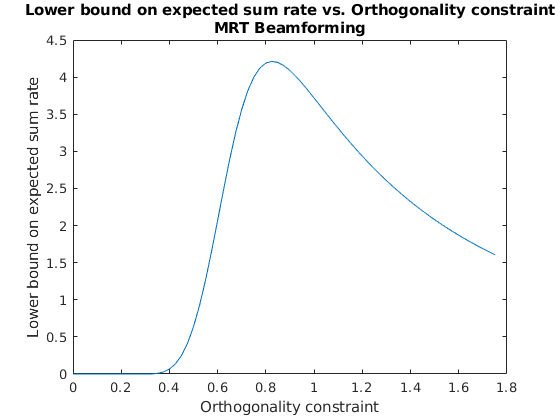
\includegraphics[width=18cm]{figs/100_candidate_mrt.png}\\
    \caption{Sum rate for two-dimensional constellations as a function of pairwise orthogonality requirement between user channels in a given group. Four users per group is assumed, four transmit antennas assumed. Number of candidate STAs for addition to SUS groups is set to 100. SNR 10dB.}
    \label{fig:100_candidate}
\end{figure}

\begin{figure}
    \centering
    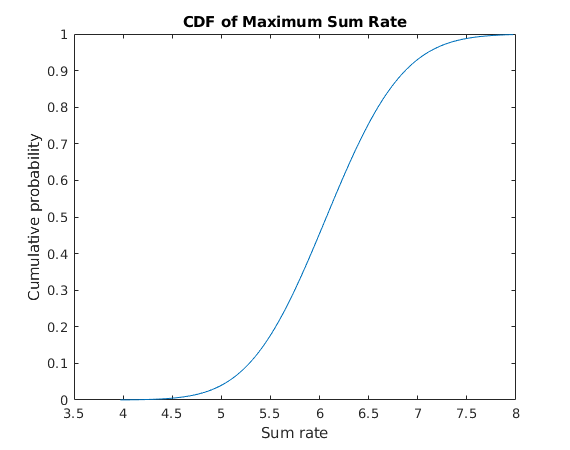
\includegraphics[width=18cm]{figs/cdf_4gs_100cand_1Ptx_0_1Pn.png}\\
    \caption{CDF of maximum sum rate for two-dimensional constellations resulting from exhaustive search of all combinations of user groups chosen from the set of candidate users.  Four users per group is assumed, four transmit antennas assumed. Number of candidate STAs for addition to SUS groups is set to 100. SNR 10dB.}
    \label{fig:100_candidate_cdf}
\end{figure}

\begin{figure}
    \centering
    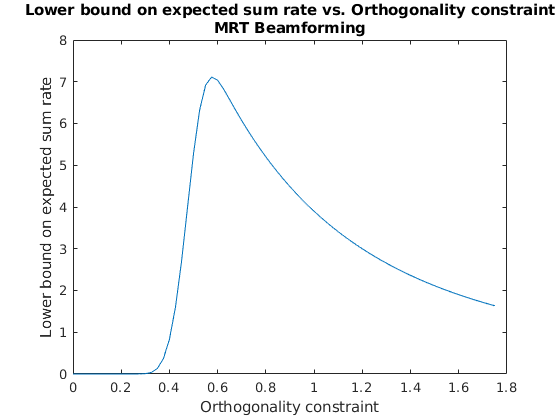
\includegraphics[width=18cm]{figs/1000_candidate_mrt.png}\\
    \caption{Sum rate for two-dimensional constellations as a function of pairwise orthogonality requirement between user channels in a given group. Four users per group is assumed, four transmit antennas assumed. Number of candidate STAs for addition to SUS groups is set to 1000. SNR 10dB.}
    \label{fig:1000_candidate}
\end{figure}

\begin{figure}
    \centering
    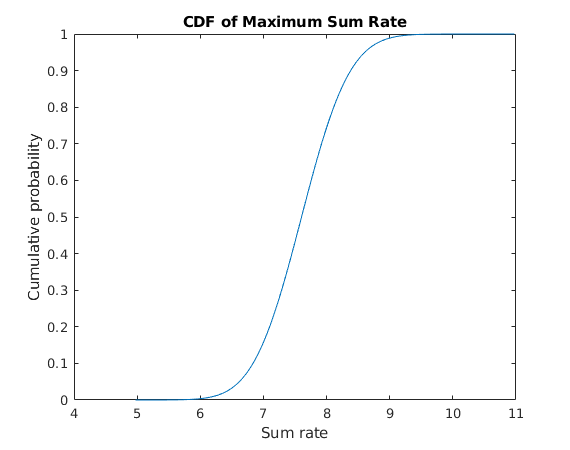
\includegraphics[width=18cm]{figs/cdf_4gs_1000cand_1Ptx_0_1Pn.png}\\
    \caption{CDF of maximum sum rate for two-dimensional constellations resulting from exhaustive search of all combinations of user groups chosen from the set of candidate users.  Four users per group is assumed, four transmit antennas assumed. Number of candidate STAs for addition to SUS groups is set to 1000. SNR 10dB.}
    \label{fig:1000_candidate_cdf}
\end{figure}
%	\section{Gaussian approximation of sum rate}
%	    \input{clt.tex}
%	\section{Maximum of normal distribution under constant mean, variance, correlation}
%	    \input{tong.tex}
%	\section{Calculation, justification of constant mean, variance and correlation}
%	    \input{const_approx.tex}
    \newpage	
 	\begingroup
 		\renewcommand{\section}[2]{}%
 		\bibliographystyle{IEEEtran}
 %		\bibliography{references}
 	\endgroup
\end{document}